\section{Semiclassical Theory of Conduction I}

\subsection{Semiclassical QM in Crystals}
We start with a wave packet with $\Delta x \Delta p \geq \hbar$, $\psi(\v{r}, t) = \sum_\v{k} g(\v{k})e^{i\v{k} \cdot \v{r} - \frac{\hbar^2 \v{k}^2}{2m}t}$. By considering the ``center of mass'' of the wave packet, we are able to derive equations of motion from the Schrodinger Equation (non-trivially) - In free space, these read:
\begin{equation}
    \begin{split}
        \dod{\v{r}}{t} &= \frac{\hbar \v{k}}{m}
        \\ \hbar \dod{\v{k}}{t} &= -e(\v{E} + \frac{1}{c}\v{v} \times \v{H})
    \end{split}
\end{equation}

In a periodic crystal, we need to revise this slightly; we have a ``wave packet'' described by Bloch wavefunctions, $\psi(\v{r}, t) = \sum_\v{k}g(\v{k})\psi_{n\v{k}}(\v{r})e^{-i\e_n(t)t/\hbar}$ where $\psi_{nk}(\v{r})$ are the Bloch eigenstates. In this setting, we obtain the equations of motion:
\begin{equation}\label{eq-crystalEOM}
    \begin{split}
        \v{v}(\v{k}) &= \frac{1}{\hbar}\nabla_\v{k} \e_n(\v{k})
        \\ \hbar\dod{\v{k}}{t} &= -e(\v{E} + \frac{1}{c}\v{v}\times \v{H}) 
    \end{split}
\end{equation}

Note that although crystal momentum is not equal to the actual momentum, we have:
\begin{equation}
    \nabla_\v{k} \e_\v{k} = \frac{\hbar^2}{2m} \int d\v{r} \psi_{nk}^* (-i\nabla)\psi_{nk}
\end{equation}
where the expectation value of velocity appears on the RHS. So, we can apply Eq. \eqref{eq-crystalEOM} if we suppose some localization in $k$-space, i.e. $\nabla k \ll \frac{1}{a}$. Note that in this limit that due to the uncertainty relation $\Delta x \Delta k \geq 1$, we have that $\Delta x \gg a$, i.e the particle is very spread out in position space.

\subsection{Limits of Validity}
We assume that electrons stay in one band, and that $\v{E}, \v{B}$ vary slowly:
\begin{equation}
    \begin{split}
        e \abs{\v{E}} a &\ll \frac{\Delta^2}{\e_F}
        \\ \hbar \omega_c &\ll \frac{\Delta^2}{\e_F}
        \\ \hbar \omega_{AC} &\ll \frac{\Delta^2}{\e_F}
    \end{split}
\end{equation}
here $\Delta$ is the band gap, $a$ the lattice spacing, and $\omega_C = \frac{eB}{m^* c}$ is the cyclotron frequency.

Note that typically $\abs{\v{E}} \sim 1\si{N.m^{-1}}$, so with $a \sim 10^{-10}\si{m}$, in order for the condition to hold we require $\Delta \gg 10^{-5}\si{eV}$. In contrast, $\abs{\v{B}} \sim 1\si{T}$ typically, where then $\hbar \omega_c \sim 10^{-4}\si{eV}$ which requires $\Delta \gg 10^{-2}\si{eV}$. So, the semiclassical approximation breaks down due to the magnetic field (known as magnetic breakdown).

\subsection{Filled Bands are Inert}
Let us define the current:
\begin{equation}
    \v{j} = (-e)\sum_{k < k_F} \v{v}(\v{k}) = -e \int_{k < k_F} \frac{d^3k}{(2\pi)^3}\frac{1}{\hbar}\nabla_{\v{k}}\e_{\v{k}}
\end{equation}
From this, we observe that filled bands are inert; looking for example at the one-dimensional case:
\begin{equation}
    \v{k} = -e\int_{k < k_F}\frac{dk}{2\pi}\frac{1}{\hbar}\dpd{}{k}\e_k = \left.\frac{e}{2\pi \hbar} \e_k \right|_{-\pi/2}^{\pi/2} = 0
\end{equation}
where the last equality is obtained via periodicity. From this observation, we would conclude that only bands near the Fermi surface are relevant for transport properties (as far as the semiclassical approximation is concerned) - filled bands will never contribute, due to this periodicity.

\subsection{Motion in a Uniform Electric Field}
For uniform $\v{E}$, we have:
\begin{equation}
    \hbar \dod{\v{k}}{t} = -e\v{E}
\end{equation}
which is immediately solved to be:
\begin{equation}
    \v{k}(t) = \v{k}(0) - \frac{e\v{E}t}{\hbar}
\end{equation}
so in time we have a displacement of $\v{k}$-values, and at a certain time, the filled states fully ``pass through'' - the below sketch illustrates this in the 1-dimensional case:

\begin{figure}[htbp]
    \centering
    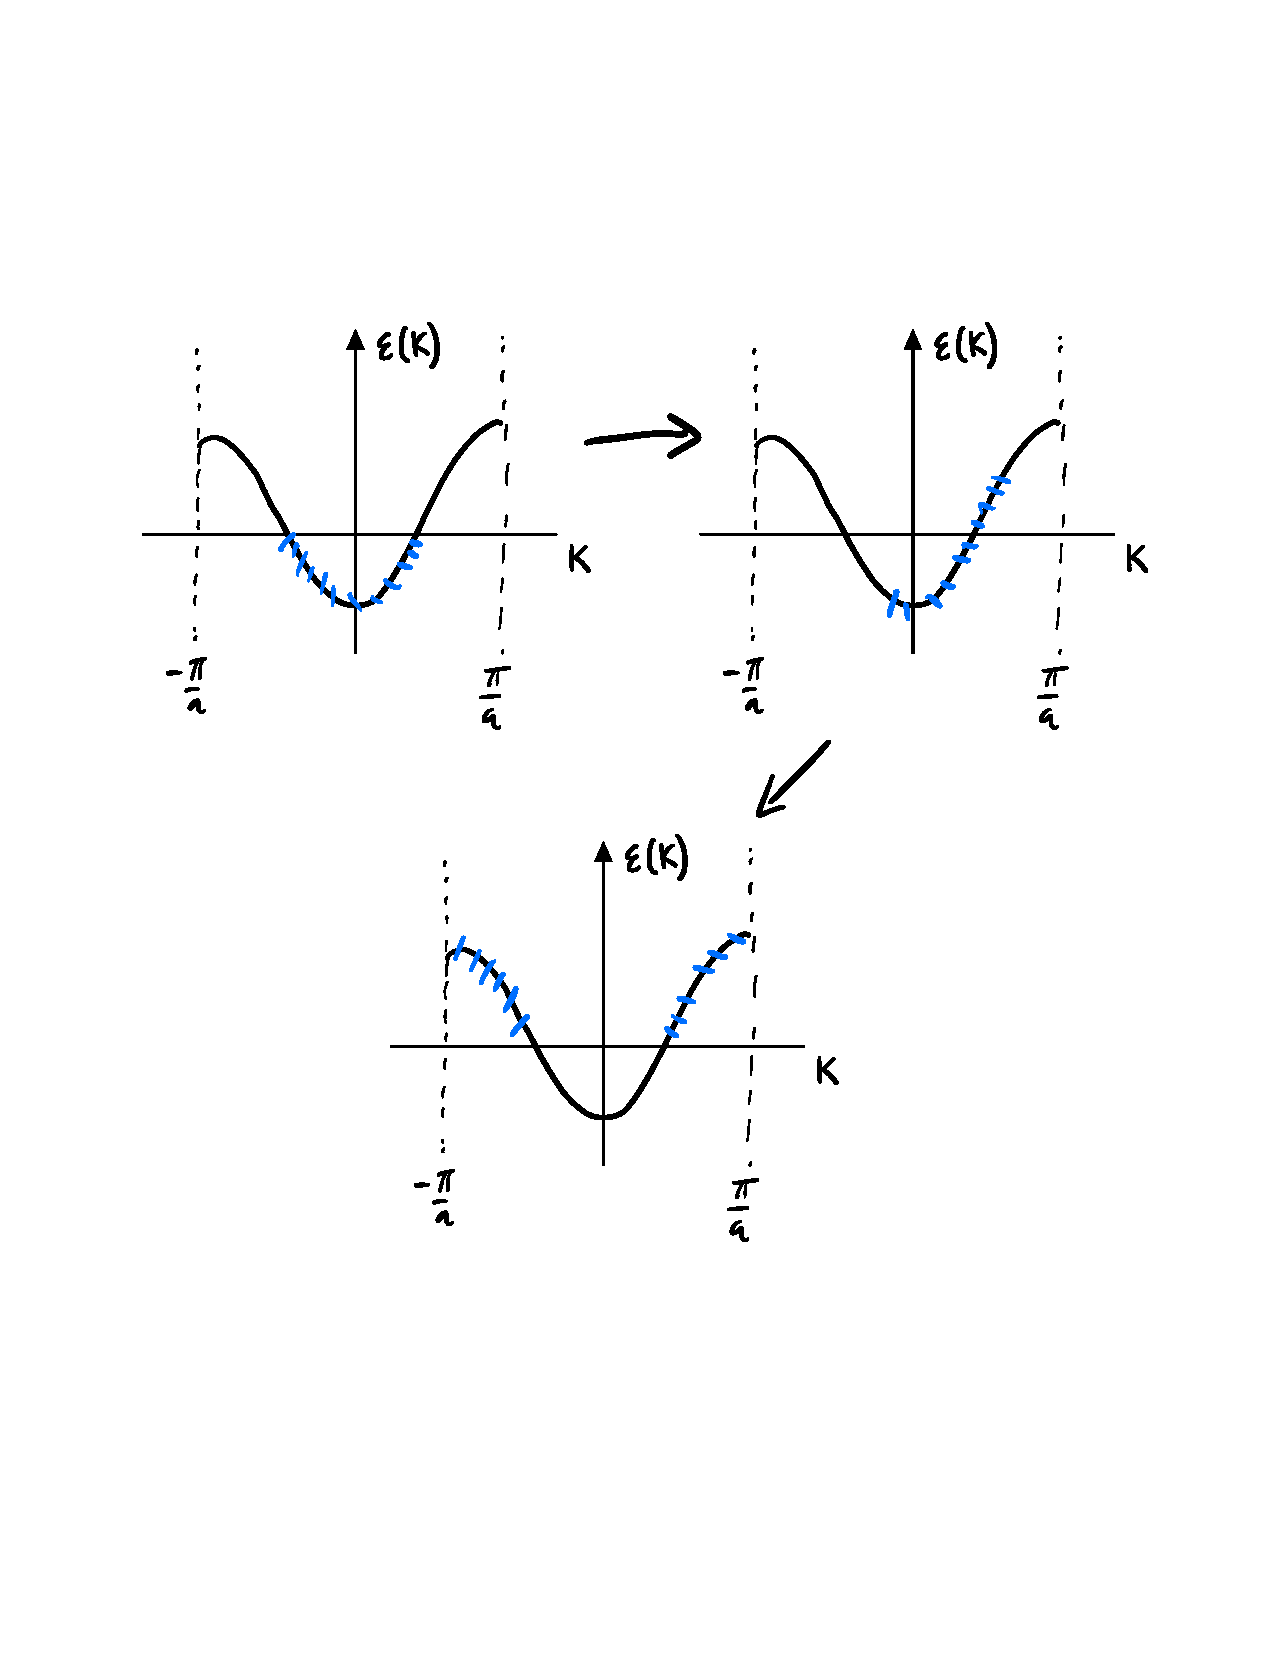
\includegraphics[scale=0.5]{Images/fig-unifEkt.pdf}
    
    \caption{1-dimensional cartoon of the displacement of $\v{k}$ values in time as a result of a uniform $\v{E}$-field.}
    \label{fig-unifEkt}
\end{figure}

Hence, since $\v{v}(t) = \v{v}(\v{k}(t)) = \v{v}(\v{k}(0) - \frac{e\v{E} t}{\hbar})$ and at some time the filled levels ``pass through'', we have oscillatory electrons/AC current!

Note in a real crystal, this phenomena does not actually occur due to electron collisions that relax $\v{v}(t)$. These break the periodicity that the Bloch wavefunctions have - in a metal these symmetry-breaking components may be phonons, impurities etc.

\subsection{The Hole Picture}
Let us rearrange the (vanishing) integral over the full band we had from our previous calculation, by splitting it into two parts:
\begin{equation}
    0 = -e\int_{\text{full band}}\frac{d^3k}{(2\pi)^3}\v{v}(\v{k}) = -e\int_{\text{occupied}} \frac{d^3k}{(2\pi)^3}\v{v}(\v{k}) + (-e)\int_{\text{unoccupied}}\frac{d^3k}{(2\pi)^3}\v{v}(\v{k})
\end{equation}
From this we obtain an equivalent way of describing the current:
\begin{equation}
    \v{j} = +e\int_{\text{unoccupied}}\frac{d^3k}{(2\pi)^3}\v{v}(\v{k})
\end{equation}
which describes the current in terms of positive charge carriers corresponding to the unoccupied parts of the band. This has practical use (e.g.) for a band which is mostly filled - where it is much easier to compute with the unoccupied states, rather than the occupied ones.

\begin{figure}[htbp]
    \centering
    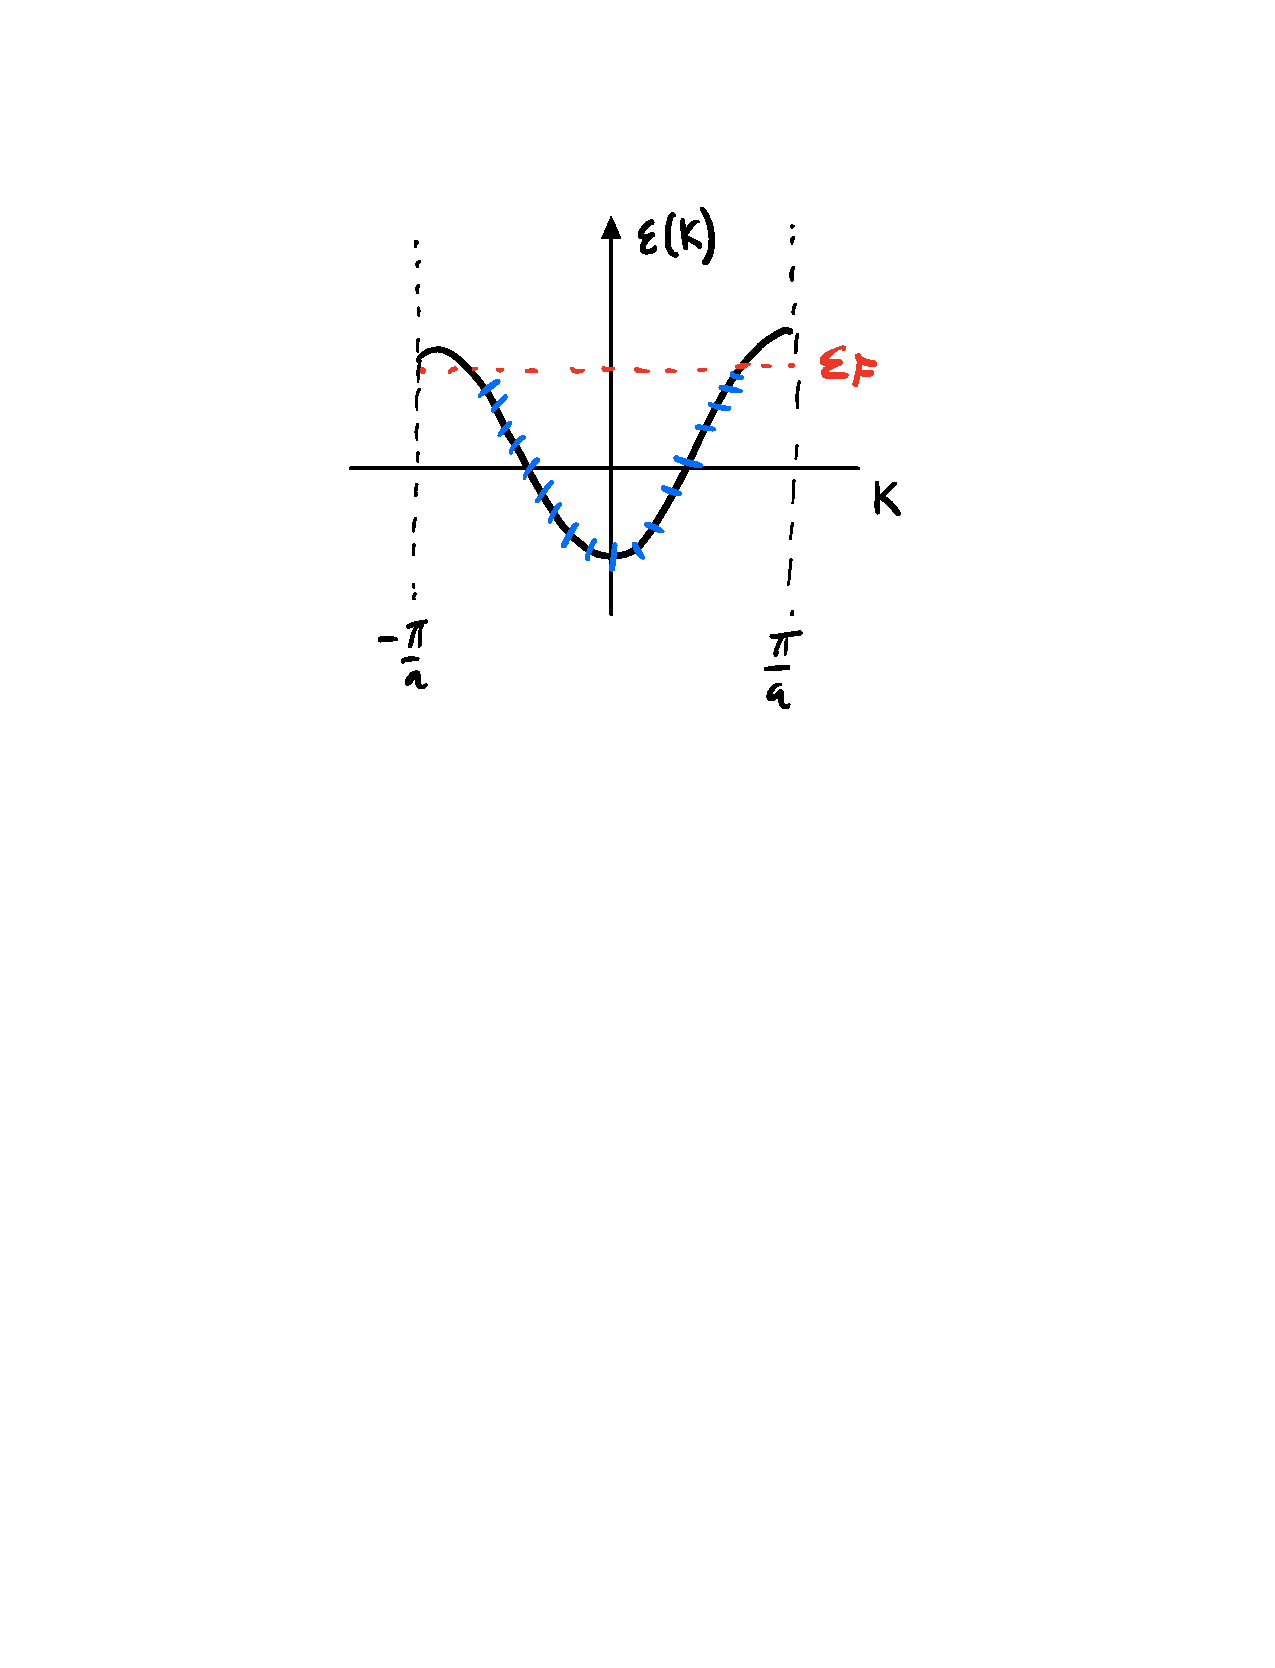
\includegraphics[scale=0.7]{Images/fig-mostlyfilledband.pdf}
    \caption{A sketch of a mostly filled band, for which the hole picture would be more convenient to do calculations in.}
    \label{fig-mostlyfilledband}
\end{figure}

\subsection{Motion in Uniform Magnetic Field}
We now consider a scenario with a uniform $\v{H}$-field (and zero electric field). We then have:
\begin{equation}
    \hbar\dod{\v{k}}{t} = -e(\v{v} \times \v{H})
\end{equation}
With $\e_\v{k} = \frac{\hbar^2(k_x^2 + k_y^2)}{2m}$, we have that $\v{v} = \frac{1}{\hbar}\nabla_{\v{k}} \e_{\v{k}} = \frac{1}{\hbar}\frac{\hbar^2}{m}(k_x, k_y) = \frac{\hbar}{m}(k_x, k_y)$ (Note: $\v{k}$ moves through state space, but $\v{v}$ is the real motion of velocity!). From this it follows that:
\begin{equation}
    \dod{\v{k}}{t} \sim \v{v} \cdot \gv{\theta}
\end{equation}
where $\gv{\theta}$ is some tangential vector.  So, the electrons will move on intersections of constant $\e_{\v{k}}$ and surfaces perpendicular to $\v{H}$!